\chapter{Numerical differencing techniques}
\label{chap:numdiff}

Several different numerical differencing techniques were studied for this report. The Taylor expansion method was used to derive the forward, reverse and centre differencing techniques, while the built-in IDL numerical differencing technique (\textsc{deriv}) uses a three-point Lagrangian technique. 

A Taylor series is the expansion of the real function $f(t)$ about the point $t=a$ and generally takes the form
\begin{equation}
f(t) = f(a) + f'(a)(t-a) +  \frac{f''(a)}{2!}(t-a)^{2} + \frac{f'''(a)}{3!}(t-a)^{3}  + ...
\end{equation}
The difference between points $(t-a)$ is defined as $\Delta t$. This expansion can be used to determine the numerical derivative of a given point using a variety of different methods, each of which is outlined in the following sections.


% Numerical Differencing Techniques

\section{Forward differencing}
\label{sect:forward}

The forward differencing technique involves the computation of the derivative at the point $t + \Delta t$ by extrapolating forward from the point $t$. This uses the Taylor series:
\begin{equation}
r(t + \Delta t) = r(t) + r'(t)\Delta t +  \frac{r''(t)}{2!}(\Delta t)^{2} + \frac{r'''(t)}{3!}(\Delta t)^{3}  + ...
\end{equation}
This equation can be re-arranged to give
\begin{equation}
r'(t)\Delta t = r(t + \Delta t) - r(t) -  \frac{r''(t)}{2!}(\Delta t)^{2} - \frac{r'''(t)}{3!}(\Delta t)^{3}  + ...
\end{equation}
which then gives
\begin{equation}
r'(t) = \frac{r(t + \Delta t) - r(t)}{\Delta t} -  \frac{r''(t)}{2!}(\Delta t) - \frac{r'''(t)}{3!}(\Delta t)^{2}  + ...
\end{equation}
This is usually written as
\begin{equation}
r'(t) = v = \frac{r(t + \Delta t) - r(t)}{\Delta t} + O(\Delta t)
\end{equation}
where $O(\Delta t)$ is the truncation error term, determined by the distance between neighbouring points ($\Delta t$). This technique assumes a straight line gradient between points. 

This estimate of the velocity is dependent on the initial units used for the distance. In the case of the simulation work done here, the units of distance are mega-metres (1~Mm = $10^6$~m). This produces an estimate of velocity in units of Mm~s$^{-1}$. To convert this to acceptable units of km~s$^{-1}$ requires multiplying the estimated velocity values by $10^{3}$. This has been done in all plots showing the numerically derived velocity. Similarly, converting the acceleration from units of Mm~s$^{-2}$ requires multiplying the estimated acceleration values by $10^{6}$.

%The forward-difference technique may be used to obtain the velocity and acceleration of the data numerically, without the use of fits. If the data can be modeled as a linear function of the form $r(t) = r_0 + v_0 t$, with a noise term of the form $\delta r$ added to the distance data (i.e.:\ $r(t) = r_0 + v_0 t + \delta r$), the velocity of the data can be estimated as
%\begin{equation}
%v = v_{0} + \frac{\delta r_{(t + \Delta t)} - \delta r_{t}}{\Delta t}
%\end{equation} 
%In this case, the velocity is estimated as the initial velocity $v_0$ with a correction term that accounts for the variation in the original data-set due to noise. This correction term is unique to each data-point due to the random nature of the applied noise.

It is possible to derive the value of the truncation error term in terms of the original $r(t)$ values. The truncation error is given as
\begin{equation}
O(\Delta t) = \frac{r''(t)}{2!}(\Delta t)
\end{equation}
The $r''(t)$ term may be decomposed using the original forward-difference definition:
\begin{equation}
r''(t) = \frac{r'(t + \Delta t) - r'(t)}{\Delta t}
\end{equation}
Rewriting each term using the original functional forms produces
\begin{equation}
O(\Delta t) = \frac{r(t + 2\Delta t) - 2r(t + \Delta t) + r(t)}{2!\Delta t}
\end{equation}
The error term associated with the velocity estimate using the forward-difference technique is therefore dependent on the value of the function $r(t)$ at the points $t$, $t+\Delta t$ and $t+2\Delta t$.

This equation must be modified when dealing with the error associated with the acceleration estimate. In this case, the truncation error term would be given as:
\begin{equation}
O(\Delta t) = \frac{v(t + 2\Delta t) - 2v(t + \Delta t) + v(t)}{2!\Delta t}
\end{equation}
Here, the velocity function $v(t)$ is treated as the base function, rather than the distance function $r(t)$ as above. 

The forward-difference technique is a very simplistic technique that produces spiky plots, with large variation between points. This is a result of the inherent assumption made by the forward-difference technique that there is a straight-line gradient between points. In addition, the forward-difference technique removes a point from the end of the data-set with each differentiation due to the way it calculates the derivative.
\section{Reverse differencing}
\label{sect:reverse}

A similar method to the forward difference method is the reverse differencing technique. In this case, the derivative at the point $t - \Delta t$ is estimated by extrapolating backwards from the point $t$, rather than forwards (hence the name). This method again uses the Taylor series:
\begin{equation}
r(t - \Delta t) = r(t) - r'(t)\Delta t +  \frac{r''(t)}{2!}(\Delta t)^{2} - \frac{r'''(t)}{3!}(\Delta t)^{3}  + ...
\end{equation}
This equation can be re-arranged to give
\begin{equation}
r'(t)\Delta t = r(t ) - r(t - \Delta t) +  \frac{r''(t)}{2!}(\Delta t)^{2} - \frac{r'''(t)}{3!}(\Delta t)^{3}  + ...
\end{equation}
which then gives
\begin{equation}
r'(t) = \frac{r(t ) - r(t - \Delta t)}{\Delta t} +  \frac{r''(t)}{2!}(\Delta t) - \frac{r'''(t)}{3!}(\Delta t)^{2}  + ...
\end{equation}
This is usually written as
\begin{equation}
r'(t) = v = \frac{r(t ) - r(t - \Delta t)}{\Delta t} + O(\Delta t)
\end{equation}
where $O(\Delta t)$ is the truncation error term which, as with the forward difference method, is determined by the distance between neighbouring points ($\Delta t$), assuming a straight line gradient between points.

The units of the velocity estimate produced using this method once again depend on the units used for the distance. The velocity estimate produced using this method must again be multiplied by $10^{3}$ to give an estimate of velocity in units of km~s$^{-1}$, while the acceleration estimate must be multiplied by $10^{6}$ to give an estimate in units of m~s$^{-2}$. As with the forward-difference technique, this has been done for all plots showing the velocity derived numerically using the reverse-difference technique.

Once again, the truncation error can be estimated in terms of the original distance function $r(t)$. The truncation error is defined as:
\begin{equation}
O(\Delta t) = \frac{r''(t)}{2!}(\Delta t)
\end{equation}
Using the definition of the reverse-difference technique, the $r''(t)$ term may be defined as
\begin{equation}
r''(t) = \frac{r'(t ) - r'(t - \Delta t)}{\Delta t}
\end{equation}
It is possible to re-write each term using the the original functional form and the definition of the reverse-difference technique. When this is done, and the values substituted into the equation for the truncation error term, this produces
\begin{equation}
O(\Delta t) = \frac{r(t) - 2r(t - \Delta t) + r(t - 2\Delta t)}{2!\Delta t}
\end{equation}
This shows a similar form to the truncation error estimate for the forward-difference technique. Both techniques are quite similar and it is not unexpected that they should show a similar form for the truncation error estimate. However, despite the similar form, the two estimates are not necessarily equal.

As before, this equation can be modified to find the truncation error associated with the acceleration term by taking the velocity function $v(t)$ as the base function rather than the distance function $r(t)$. When this is done, this produces a truncation error of:
\begin{equation}
O(\Delta t) = \frac{v(t) - 2v(t - \Delta t) + v(t - 2\Delta t)}{2!\Delta t}
\end{equation}

Both the forward and reverse difference techniques are very similar and use two adjacent points ($t$ \& $t+\Delta t$ and $t$ \& $t-\Delta t$ respectively) to find the derivative at a chosen point. They are both very simplistic techniques and are only applicable in very simplistic cases. The reverse-difference technique is also observed to remove a point from the beginning of the data-set with each numerical derivative due to the way the technique is calculated. 


\section{Centre differencing}
\label{sect:centre}

A more accurate technique using the Taylor expansion method is the centre difference technique. This uses the points either side of the point under examination $t$ (i.e..:\ $t - \Delta t$ and $t + \Delta t$), smoothing the data and producing a more accurate estimate of the numerical derivative at that point. From above, the Taylor series expansion is defined as
\begin{equation}
r(t - \Delta t) = r(t) - r'(t)\Delta t +  \frac{r''(t)}{2!}(\Delta t)^{2} - \frac{r'''(t)}{3!}(\Delta t)^{3}  + ...
\end{equation}
at the point $t - \Delta t$ and 
\begin{equation}
r(t + \Delta t) = r(t) + r'(t)\Delta t +  \frac{r''(t)}{2!}(\Delta t)^{2} + \frac{r'''(t)}{3!}(\Delta t)^{3}  + ...
\end{equation}
at the point $t + \Delta t$. The centre differencing technique subtracts the following point from the leading point:
\begin{equation}
r(t + \Delta t) - r(t - \Delta t)
\end{equation}
This produces the equation
\begin{equation}
r(t + \Delta t) - r(t - \Delta t) = 2 r'(t)\Delta t +  2 \frac{r'''(t)}{3!}(\Delta t)^{3}  + ...
\end{equation}
This equation can then be re-arranged to give
\begin{equation}
r'(t) = \frac{r(t + \Delta t) - r(t - \Delta t)}{2 \Delta t} - \frac{r'''(t)}{3!}(\Delta t)^{2}  + ...
\end{equation}
Following the notation from before, this is usually written
\begin{equation}
r'(t) = \frac{r(t + \Delta t) - r(t - \Delta t)}{2 \Delta t} + O(\Delta t^{2})
\end{equation}
where $O(\Delta t^{2})$ is the truncation error term. The truncation error term in this case is determined by the square of the distance between neighbouring points, producing a more accurate estimate than the forward and reverse difference methods. 

As with the forward and reverse-difference techniques, the velocity estimate produced by the centre-difference method must be multiplied by $10^{3}$ to give the physically realistic units of km~s$^{-1}$, with the acceleration estimate multiplied by $10^{6}$ to give the physically realistic units of m~s$^{-2}$. This has been done for all the simulated data-sets that have been processed using the centre-difference technique.

%\begin{figure}[!t] 
%  \centerline{
%              \includegraphics[width=0.9\textwidth,trim = 0mm 0mm 0mm 0mm,clip=]{images/c_diff_lin.eps}
%              }
%\caption[Centre difference technique simulation]{\emph{Top}: Simulated distance-time data with noise added. \emph{Middle}: Velocity-time data obtained using a centre-difference technique. \emph{Bottom}: Acceleration-time data obtained using a centre-difference technique. }
%\label{fig:c_diff_sim}
%\end{figure}

The centre-difference method effectively smoothes the data set while differentiating it by using the two points either side of the point under examination. The truncation error can once again be given in terms of the original function. From above the truncation error is defined as:
\begin{equation}
O(\Delta t^{2}) = \frac{r'''(t)}{3!}(\Delta t)^{2}
\end{equation}
In this case, the truncation error is defined by the third order derivative of the original function (unlike the second-order derivative for the forward and reverse-difference methods). As before, the third-order derivative can be defined as
\begin{equation}
r'''(t) = \frac{r''(t + \Delta t) - r''(t - \Delta t)}{2 \Delta t} 
\end{equation}
using the definition of the centre-difference technique. Once all of the terms have been re-written in terms of the original equation, the truncation error term, may be written as
\begin{equation}
O(\Delta t^{2}) = \frac{r(t + 3\Delta t) - 3r(t + \Delta t) + 3r(t - \Delta t) - r(t - 3\Delta t)}{(3!)(8)\Delta t}
\end{equation}
This produces a mean truncation error estimate that is much smaller than the mean truncation error calculated using the forward and reverse-difference techniques.

As with the forward and reverse-difference techniques, the truncation error term can be estimated for the acceleration term by using the velocity function $v(t)$ as the base function rather than the distance function $r(t)$. When this is done, it produces the estimate
\begin{equation}
O(\Delta t^{2}) = \frac{v(t + 3\Delta t) - 3v(t + \Delta t) + 3v(t - \Delta t) - v(t - 3\Delta t)}{(3!)(8)\Delta t}
\end{equation}
for the truncation error of the acceleration data. 

The centre-difference technique produces a mean truncation error estimate and a scatter in the data that are much smaller than the forward and reverse-difference techniques. As a result, the centre-difference technique produces a better estimate of the velocity and acceleration, and their associated truncation errors than either the forward or reverse-difference techniques.
\section{Lagrangian differentiation}
\label{sect:lagrange}

%\begin{figure}[!t] 
%  \centerline{
%              \includegraphics[width=0.9\textwidth,trim = 0mm 0mm 0mm 0mm,clip=]{images/l_diff_lin.eps}
%              }
%\caption[Lagrange difference technique simulation]{\emph{Top}: Simulated distance-time data with noise added. \emph{Middle}: Velocity-time data obtained using a three-point Lagrange difference technique. \emph{Bottom}: Acceleration-time data obtained using a three-point Lagrange difference technique. }
%\label{fig:l_diff_sim}
%\end{figure}

A more advanced numerical differentiation method is the three-point Lagrangian method used by the \textsc{deriv} routine in IDL. This method uses three adjacent points ($t-\Delta t$, $t$ and $t+\Delta t$) to fit a Lagrange polynomial function of the form
\begin{eqnarray}
P(x) &=& \frac{(x - t)(x - (t+\Delta t))}{((t-\Delta t) - t)((t-\Delta t)- (t+\Delta t))}y_{1} \nonumber \\
&+& \frac{(x - (t-\Delta t))(x - (t+\Delta t))}{(t - (t-\Delta t))(t - (t+\Delta t))}y_{2} \nonumber \\ 
&+& \frac{(x - (t-\Delta t))(x - t)}{((t+\Delta t) - (t-\Delta t))((t+\Delta t) - t))}y_{3}
\end{eqnarray}
to the three points, and hence find the derived value at a point numerically.

This method gives a more accurate indication of the numerically differentiated data as it does not assume a straight line in between points. In addition, the routine compensates for edge points, increasing the errors of the points. It also uses three points to find the numerical derivative, rather than two (c.f. centre, forward and reverse-difference techniques). The Lagrangian technique also smoothes the data-set, removing the spiky appearance that arises from use of the different Taylor series techniques.

\begin{deluxetable}{ccc}
\tablecolumns{3}
\tabletypesize{\small}
\tablewidth{0pt}
\centering
\tablecaption{Numerical differentiation errors \label{tbl:numdiff}}
\tablehead{
\colhead{Method} & \colhead{Kinematics} & \colhead{Error term}
}
\startdata
Forward diff. & Velocity &  $O(\Delta t) = \frac{r(t + 2\Delta t) - 2r(t + \Delta t) + r(t)}{2!\Delta t}$  \\
 & Acceleration & $O(\Delta t) = \frac{v(t + 2\Delta t) - 2v(t + \Delta t) + v(t)}{2!\Delta t}$   \\
Reverse diff. & Velocity &  $O(\Delta t) = \frac{r(t) - 2r(t - \Delta t) + r(t - 2\Delta t)}{2!\Delta t}$   \\
 & Acceleration & $O(\Delta t) = \frac{v(t) - 2v(t - \Delta t) + v(t - 2\Delta t)}{2!\Delta t}$   \\
Centre diff. & Velocity & $O(\Delta t^{2}) = \frac{r(t + 3\Delta t) - 3r(t + \Delta t) + 3r(t - \Delta t) - r(t - 3\Delta t)}{(3!)(8)\Delta t}$   \\
 & Acceleration & $O(\Delta t^{2}) = \frac{v(t + 3\Delta t) - 3v(t + \Delta t) + 3v(t - \Delta t) - v(t - 3\Delta t)}{(3!)(8)\Delta t}$   \\
Lagrangian & Velocity & $\sigma$  \\
 & Acceleration & $\sigma$  \\
\enddata
\end{deluxetable}

 The problems encountered in this work arise from the small data-sets available in the case of these disturbances. The small data-sets mean that there are only four or five points available of which three are needed to calculate the numerical derivative of each point. This makes the Lagrangian technique unsuitable for estimating the kinematics of these disturbances.

The three-point Lagrangian interpolation method used by IDL uses the standard deviation of the derivative calculated by the Lagrangian polynomial as the truncation error of the numerical derivative. This produces a consistent estimate of the mean truncation error that only varies with the end-points due to the increased uncertainty of these points.

Table~\ref{tbl:numdiff} shows the different estimates for the truncation error term for each numerical differencing technique. These truncation error estimates are given in terms of the original base function, the exception being for the Lagrangian technique, which takes the standard deviation of the Lagrange derivative at a point as the truncation error estimate at that point.


%Figure~\ref{fig:l_diff_sim} shows the three-point Lagrangian technique operating on the simulated data-set used for the forward, reverse and centre difference methods. This figure has the same scaling as Figures~\ref{fig:f_diff_sim} to \ref{fig:c_diff_sim} to show the difference in errors between the different methods. The Lagrangian technique has much lower errors than the forward or reverse difference methods, and also smaller errors than the centre difference method. The errors are comparable with the data itself, but are still much larger than is reasonable for accurate data analysis. The Lagrangian method also has a problem with the edges of numerically derived data, and often drags these points downwards. This can result in false conclusions being made about the derived data.


% Kinematical model for the simulation work

\input{models}

% Discussion and explanation of the application of noise for the simulation

\input{noise}

% Presentation and analysis of the simulations

\input{sim_and_analysis}
